%!TEX root=rapport.tex

\subsection{Alignement}
\label{subsection:alignment}

Les deux dernières étapes que sont l'alignement et le consensus sont
implémentées dans la classe \verb|ConsensusAbstract| à travers les méthodes
\emph{computeAlignment} qui calculent l'alignement des séquences et le sauvegardent
dans l'attribut \emph{alignment} ainsi qu'à travers la méthode \emph{build}
qui calcule le consensus.

Pour calculer l'alignement, nous utilisons les segments alignés dans l'ordre
donné par l'algorithme glouton décrit à l'étape \ref{subsection:greedy}.
Cet algorithme nous donne une liste de paires de séquences $P_{i}$ telles
que le deuxième segment de la paire $P_{i}$ provient du même segment initial que
le premier de la paire $P_{i + 1}$, la différence entre ces deux séquences se
situant dans les gaps ajoutés lors de l'alignement semi-global entre les
nucléotides pour offrir le meilleur score pour chaque paire.

%\todo{Insérer un exemple de la sortie du greedy.}

Pour pouvoir construire le contig final, il nous faut réaligner convenablement
chaque paire de segments et, pour cela, nous propageons les gaps qui ont été
ajoutés lors des calculs de l'alignement semi-global. Nous effectuons cette
propagation en deux temps:

\begin{enumerate}
	\item vers le bas, c'est-à-dire, pour une paire $P_{i}$, nous regardons si
		entre deux nucléotides de la deuxième composante de $P_{i}$, le nombre
		de gaps est plus grand qu'entre les deux mêmes nucléotides de la
		première séquence de la paire suivante $P_{i + 1}$. Si c'est le cas,
		nous propageons la différence entre ces nombres vers les séquences du
		dessous.
	\item vers le haut par le même procédé que pour la propagation vers le bas
		si ce n'est que nous propageons les gaps qui sont plus présents dans la
		première composante de la paire $P_{i + 1}$ que dans la deuxième
		composante de paire $P_{i}$ et que nous propageons alors la différence
		de gaps vers les séquences du dessus.
\end{enumerate}

%\todo{Insérer un exemple d'après propagation.}

Si nous posons $P_{i} = (s_{i}, t_{i})$, ce procédé nous permet d'être sûr que
les séquences $t_{i}$ et $s_{i + 1}$ sont bien les mêmes et alignées car les
gaps insérés lors des alignements semi-globaux ont été propagés dans ces deux
séquences.

Avant de décrire les algorithmes, nous introduisons une nouvelle abstraction des
séquences qui facilitera la propagation des gaps, que cela soit au niveau
complexité mémoire ou complexité temps qu'au niveau de l'implémentation des
algorithmes de propagations.

\subsubsection{Représentation d'une séquence pour l'alignement}
\label{subsubsection:repr_sequence_alignment}

Au vu de la méthode de propagation de gaps utilisée, le procédé d'alignement
consiste en un ajout de gaps entre nucléotides: il est dès lors intéressant de
représenter les séquences alignées comme des séquences sans gaps où, après
chaque nucléotide de la séquence, nous retenons, dans un tableau d'entiers, le
nombre de gaps suivant celui-ci.\footnote{Une même représentation peut être
	utilisée pour représenter pour les nucléotides successifs identiques: nous
	compressons ainsi la séquence. Nous n'avons souhaité compresser que les gaps
	car nous ne travaillons qu'avec ceux-ci, et cela aurait complexifié
l'implémentation des méthodes.}

Par exemple, la séquence \verb|A--T-G-C| est représentée par une séquence
\verb|ATGC| et par un tableau nommé \emph{nb\_gaps} de taille 4
contenant les entiers {2, 1, 1, 0} car il y a deux gaps après le premier
nucléotide, un gap après le second, un après le troisième, et 0 à la fin. Les
complexités en temps et en mémoire sont ainsi diminuées car la plupart des
algorithmes travaillent avec la séquence initiale.
Au niveau de la mémoire, une séquence alignée est alors la
séquence initiale muni d'un tableau d'entier de gaps.

L'ajout de gaps est alors simple et rapide en complexité. En effet,
si nous souhaitons ajouter un gap à la position 2 (supposons qu'on commence à
calculer en 0) à la séquence \verb|A--T-G-C| pour obtenir \verb|A---T-G-C|, il
nous suffira d'augmenter de 1 le nombre de gaps après le nucléotide A: nous
obtiendrons alors le tableau {3, 1, 1, 0}. Cet ajout de gap peut se faire en
$O(n)$ où $n$ est la taille de la séquence \textit{initiale}. De plus,
l'insertion de gaps ne demande pas plus d'espace mémoire: qu'importe le nombre
de gaps, nous ne faisons qu'augmenter la case
correspondante du tableau \emph{nb\_gaps}. \footnote{Avec la représentation sous
	forme de byte (1 octet en Java), cette nouvelle abstraction est intéressante
si nous devons ajouter plus de 7 gaps entre chaque nucléotide (ce qui ferait un
total de 8 octets, la taille que prend la nouvelle abstaction quelque soit le
nombre de gaps), ce qui peut
arriver si nous travaillons sur de grandes séquences.} La plupart des méthodes
ont alors une complexité relative à la taille de la
séquence \textit{initiale}, et non la séquence alignée et vu que l'insertion de
gaps ne modifie jamais la taille de la séquence initiale, nous
gardons toujours une complexité relative à la taille de la séquence initiale, ce
qui est avantageux dans le cas d'insertions de très grands nombres de gaps.

Un autre point positif est qu'il est très facile de connaitre la position où nous
devons insérer des gaps s'il nous est demandé de rajouter $n$ gaps entre deux
nucléotides: il suffit de connaitre la position du nucléotide dans la chaine
initiale après lequel nous devons ajouter les $n$ gaps. Ce point sera utilisé
lors de la propagation de gaps dans la section \ref{propagation_gaps}.

Nous gardons également un attribut contenant l'offset de la séquence dans le
chemin hamiltonien, c'est-à-dire le décalage vers la droite du début de la
séquence. Cela nous amène à parler de position relative et de position absolue.
La position relative d'un élément dans une séquence est la position de l'élément
sans l'offset tandis que la position absolue est la position en prenant compte
de l'offset.

\begin{exemple} [Offset]
	Supposons que l'algorithme glouton nous renvoie les alignements

	\verb|   A-TGC-|

	\verb|ATTAATGCT|

	et

	\verb|ATTAATG-CT|

	\verb|   AATGTCT|

	ce qui donne, quand nous alignons la deuxième et troisième séquence,

	\verb|   A-TGC-|

	\verb|ATTAATGCT|

	\verb|ATTAATG-CT|

	\verb|   AATGTCT|

	La deuxième et troisième séquence ont un offset de 0 (car ce sont elles qui
	sont le plus à gauche), tandis que la première et la dernière ont un offset
	de 3 car elles sont décalées de 3 vers la droite.

	Lors du calcul de l'alignement, nous devrons nous souvenir de ces offsets.
	Nous nous servirons alors de la méthode \emph{updateOffset} qui aura pour
	but de mettre à jour l'attribut offset.
\end{exemple}

\begin{exemple} [Position relative et absolue]
	Soit la séquence \verb|A--T-G-C| et considérons un offset de 4, c'est-à-dire
	que \og réellement \fg, la séquence est \verb|----A--T-G-C|.

	En commençant de calculer à 0, le nucléotide à la position relative 3 est
	\verb|T| tandis que ce même nucléotide est à la position absolue $4 + 3 = 7$,
	l'élément à la position absolue 3 étant le dernier gap avant le \verb|A|.
\end{exemple}

Cette distinction est à faire car lorsque nous devons propager des gaps (voir
\ref{propagation_gaps}), nous devons considérer cet offset, c'est-à-dire
travailler avec la position absolue.

Par la suite, nous travaillerons toujours avec la position \textit{absolue}.

Cette abstraction des séquences est implémentée dans la classe
\verb|SequenceAbstract|.\footnote{Cela justifie le nom de la classe
	\verb|ConsensusAbstract| qui travaille avec des objets de la classe
\verb|SequenceAbstract|, et non \verb|Sequence|.}

Divers constructeurs sont implémentés (pour permettre diverses compatibilités
avec les autres parties et si nous souhaitons améliorer le projet) mais un seul
est utilisé dans \verb|ConsensusAbstract|: celui qui demande un objet de la
classe \verb|Sequence| représentant une séquence alignée.  L'algorithme, en
$O(n)$ où $n$ est la taille de la séquence alignée, reconstruit la séquence
initiale et le tableau de gaps, l'offset étant mis à la position du premier
nucléotide.

Les autres méthodes utilisées sont:
\begin{description}
	\item[\emph{getSize}]: Récupère la taille de la séquence. La taille est
		contenue dans un attribut \emph{size} qui est mis à jour à chaque fois
		que nous ajoutons des éléments et cette mise à jour se fait en O(1). Cette
		implémentation permet de garder une complexité en O(1) et de diminuer la
		complexité de \emph{addEndGaps} dans \verb|ConsensusAbstract| par
		exemple.
	\item[\emph{complement}]: Construit, en $O(m)$ avec $m$ la taille de la
		séquence \textit{initiale}, le complémentaire inversé de la séquence.
		Cette méthode est donc plus rapide que la méthode \emph{complement} de
		\verb|Sequence| qui nécessite de parcourir toute la séquence
		\textit{alignée}.
	\item[\emph{addGapsAndReturnIndice}]: insère $n$ gaps à
			une position (absolue) donnée et retourne l'indice (dans la séquence
			initiale) du nucléotide après lequel les gaps ont été insérés, le
			tout en $O(m)$ où $m$ est la taille de la séquence initiale. Le
			retour de la fonction est utile pour la propagation entre deux
			séquences provenant d'une même séquence initiale quand on doit
			connaître entre quels nucléotides nous avons inséré les gaps.
	\item[\emph{addGapsAfterIndiceAndReturnPosition}]: insère $n$ gaps après
		le nucléotide se trouvant à l'indice donné dans la séquence initiale et
		retourne la position absolue où les gaps ont été insérés.
		Cette méthode est utilisée quand nous devons propager des gaps entre
		deux séquences ne provenant pas de la même séquence initiale et que nous
		devons connaitre alors la position où les gaps ont été insérés. La
		complexité est également en $O(m)$ où $m$ est la taille de la séquence
		initiale.
\end{description}

\subsubsection{Propagation des gaps}
\label{propagation_gaps}

Comme expliqué précédemment, la propagation des gaps se fait en deux temps: vers
le bas puis vers le haut.

Les méthodes s'occupant de la propagation se trouvent dans la classe
\verb|ConsensusAbstract|.

Avant tout, en se rappelant que le chemin hamiltonien retourné par le greedy ne
tient pas compte de l'offset, il faut le calculer. La méthode
\emph{computeOffset} s'occupe, en $O(k)$ où $k$ est la longueur du chemin
hamiltonien, de mettre à jour les offsets des séquences du chemin en alignant
les séquences provenant de la même séquence initiale. C'est-à-dire, pour deux
paires $P_{i}$ et $P_{i + 1}$, la deuxième séquence de $P_{i}$ va être alignée
(\emph{i.e.,} le premier nucléotide est placé au même décalage) avec la première
séquence de $P_{i + 1}$.

Viennent les propagations des gaps.
Les méthodes s'en chargeant sont
\emph{propageGapsDownFrom} et \emph{propageGapsUpFrom}. Les algorithmes étant
sensiblement les mêmes pour le bas et le haut, nous décrivons uniquement la
propagation vers le bas.

Dans \emph{computeAlignment}, nous parcourons chaque paire $P_{i}$ du chemin
hamiltonien et faisons appel à \emph{propageGapsDownFrom} en envoyant comme
paramètre l'indice $i$. Comme expliqué précédemment, il faut regarder la
séquence $t_{i}$ se trouvant en seconde position dans la paire $P_{i}$ et celle en
première position de la paire $P_{i + 1}$, notée $s_{i + 1}$, et parcourir
chaque nucléotide en propageant vers le bas la différence de gaps si $t_{i}$
comporte plus de gaps que $s_{i + 1}$. Nous rappelons que $t_{i}$ et $s_{i +
1}$ proviennent de la même séquence initiale et ont donc les mêmes nucléotides,
la différence entre ces deux séquences se situant dans le nombre de gaps entre
chacun d'entres eux.

S'il y a plus de gaps dans $t_{i}$ que dans $s_{i + 1}$ entre les
nucléotides $n_{k}$ et $n_{k + 1}$ (ce que nous pouvons savoir en $O(1)$ grâce à
la nouvelle abstraction des séquences car il suffit de comparer le tableau des
gaps à la position $k$), nous propageons la différence vers le bas.
Cette propagation se fait à travers la méthode
\emph{propageGapsDownFromPosition} (resp. \emph{propageGapsUpFromPosition}) qui
prend deux paramètres: l'indice et le nombre de gaps à propager.

Cette dernière méthode parcourt, à partir de la paire $P_{i} = (s_{i}, t_{i})$,
toutes les paires $P_{j} = (s_{j}, t_{j})$, $i < j \leq n$ et ajoute le nombre
de gaps demandés dans les segments $s_{j}$ et $t_{j}$. Supposons que nous devons
propager des gaps venant d'entre les nucléotides $n_{k}$ et $n_{k + 1}$ de
$t_{i}$, c'est-à-dire que nous devons insérer dans $s_{i + 1}$ après l'indice
$k$.

L'insertion se fait de manière récursive sur $j$:
\begin{itemize}
	\item[$\bullet$] Pour $j = i + 1$, c'est-à-dire la paire juste après $P_{i}$, nous
		devons insérer les gaps entre les deux nucléotides $n_{k}$ et $n_{k +
		1}$ de $s_{i + 1}$. Cette insertion se fait grâce à la méthode
		\emph{addGapsAfterIndiceAndReturnPosition} sur $s_{i + 1}$ (en $O(m)$,
		$m$ étant la taille de la séquence initiale d'où provient $t_{i}$) et
		nous récupérons en plus la position absolue d'insertion (ce qui génère
		le $m$ dans la complexité de la méthode car nous devons calculer à la
		volée la position absolue). Cette position absolue va permettre de
		savoir où il faut propager les gaps dans la séquence $t_{i + 1}$. Grâce
		à cette position $p$, nous utilisons la méthode
		\emph{addGapsAndReturnIndice} sur $t_{i + 1}$ pour insérer les gaps à la
		position $p$, et nous récupérons en même temps l'indice du nucléotide de
		$t_{i + 1}$ après lequel les gaps ont été ajoutés. Cette dernière
		méthode est également en $O(m)$,
		toujours pour la même raison que précédemment.
	\item[$\bullet$] Pour $j > i + 1$, nous répétons l'opération du cas de base mais cette
		fois-ci, nous utilisons l'indice que la méthode
		\emph{addGapsAndReturnIndice} nous a renvoyé à l'étape $j - 1$.
\end{itemize}

Pour un appel à \emph{propageGapsUpFromPosition}, nous obtenons donc une
complexité en $O( (k - i) M_{i})$ où $M_{i}$ est la taille de la plus grande
séquence du chemin, $k$ le nombre initial de séquence et $i$ la position de
début de l'insertion.

Cela entraine donc une complexité en $O( (k - i) M_{i}^{2})$ pour
\emph{propageGapsDownFrom} car nous faisons appel, pour chaque nucléotide de
$t_{i}$ (dans le pire des cas), à la méthode \-\emph{propageGapsUpFromPosition}.
Par conséquence, comme \emph{propageGapsDown} parcourt toutes les paires en
faisant appel à \emph{propageGapsDown}, nous obtenons une complexité finale de
$O(k^{2} M_{i}^{2})$.

Pour simplifier le calcul du consensus à la dernière étape, nous mettons à jour
les gaps finaux des séquences pour que toutes les séquences aient la même
longueur. Ce calcul est fait par \emph{addEndGaps} et se déroule en $O(k)$ où
$k$ est le nombre initial de séquences. Cette méthode se charge de calculer la
taille de la plus longue séquence (en $O(k)$ car \emph{getSize} est en $O(1)$)
et elle ajoute le nombre de gaps dans le tableau \emph{nb\_gaps} pour chaque
séquence. Ce nombre de gaps à ajouter à la séquence courante est égale à la
taille maximale moins la taille de la séquence courante.

Pour l'ensemble de la méthode \emph{computeAlignment}, on obtient donc une
complexité de

\begin{equation}
	\overbrace{O(k)}^{\text{ mise à jour offset}} + \overbrace{2 O(k^{2}
	M_{i}^{2})}^{\text{propagation haut et bas}} + \overbrace{O(k)}^{\text{ajout
	des gaps finaux}} = O(k^{2} M_{i}^{2})
\end{equation}

%TODO: exemple de propagation. En trouver un avec 3 séquences initiales pour
%montrer que la propagation ne se fait pas en colonne.
%\begin{center}
	%- - AT - - G - - C - -
%\end{center}

\subsection{Consensus}
\label{subsection:consensus}

Grâce à l'alignement précédemment réalisé, les paires $P_{i}$ et $P_{i + 1}$ ont
maintenant la même séquence respectivement en deuxième composante et en première
composante et toutes les séquences sont maintenant bien alignées. Pour
construire le contig final, nous parcourons chaque colonne de l'alignement
et prenons le nucléotide qui apparait le plus souvent. En cas d'égalité, nous
prenons par ordre alphabétique.

Pour parcourir les objets de la classe \verb|SequenceAbstract|, nous avons
implémenté un itérateur sur ceux-ci qui permet d'avoir un algorithme clair et
dont la complexité est en $O(k M_{i})$ où $k$ est le nombre initial de
séquences et $M_{i}$ la taille de la plus longue séquence.

\begin{comment}

\subsection{Deuxième approche}

Dans cette section nous expliquons l'approche du calcul de la séquence finale exposé par Aline.
L'idée est un peu différente, car au contraire de l'approche précédente, nous ne propageons pas physiquement les gaps mais travaillons sur les paires d'alignements en les parcourant de gauche à droite chacune à leur tour. Chaque paire d'alignement n'étant pas de la même longueur ni parfaitement alignés les uns en dessous des autres, il faut savoir se rappeler à quelle position de la séquence finale nous nous trouvons réellement lors du traitement. C'est ici que l'idée d'\emph{offset} intervient. Cette méthode nécessite un nouvel objet \verb|Counter| qui est un compteurr  permettant de retenir pour chaque colonne le nombre de $A$, de $C$, de $T$ et de $G$ qui ont été comptabilisés en une certaine position (pour un certain compteur) de la séquence finale. Une fois tous les compteurs récupérés pour toutes les positions de la séquence finale il suffit de récupérer le nucléotide ayant comptabilisé le maximum d'occurrences pour cette colonne.

Un premier test de l'implémentation de cette idée a été effectué sans tenir compte du fait que des gaps pouvaient apparaitre au sein même d'un alignement. Par exemple si on a l'alignement de $(f,g)$ puis celui de $(g,h)$, il se peut que les gaps internes au niveau de $g$ dans le premier alignement ne soient pas les mêmes que les gaps internes de $g$ au niveau du second alignement.
Nous avons pour cela besoin d'un dictionnaire qui a un entier (une position possible dans la séquence finale) associe un compteur et de la notion d'offset.

Pour mieux comprendre la notion d'offset, illustrons-la sur la situation de la figure~\ref{offset}. Lors du parcours de première paire d'alignement, l'offset est à 0 car $f$ est à gauche de $g$. On parcourt alors toutes les positions des deux alignements en créants de nouveaux compteurs car il n'en existe pas encore pour les positions couvertent par $f$ et $g$.
Lorsqu'on va traiter l'alignement $(g,f)$ l'offset devient négatif car le nucléotide le plus à gauche à traiter est avant le nucléotide que l'on avait considérer comme étant en position 0 (le premier nucléotide de la séquence $f$). On parcourt alors cet alignement de la gauche vers la droite sachant que pour certaine position (celles déjà couvertent par l'alignement $(f,g)$) des compteurs existent déjà et qu'il nous suffit donc de les mettre à jour.
\begin{figure}
		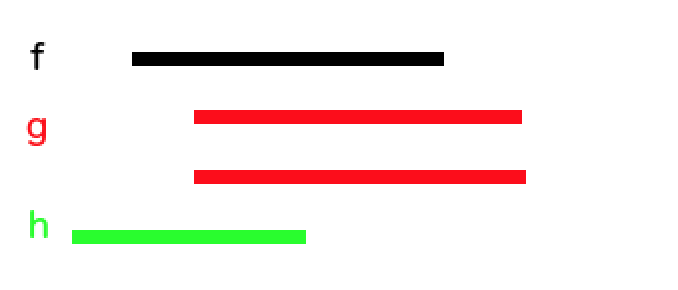
\includegraphics[scale= 0.50]{offset.png}
		\caption{Deux paires d'alignement $(f,g)$ et $(g,f)$}
		\label{fig:offset}
\end{figure}

Une telle approche, plutôt naïve, fournit déjà des résultats plutôt satisfaisants.
\end{comment}
